\chapter{Theoretische Grundlagen}
\label{ch:fundamentals}
Dieses Kapitel stellt dem Leser benötigtes Basiswissen zur Verfügung. Es wird ein grundlegendes Wissen zu den Themenbereichen \ac{DLT} und \ac{IOT} vermittelt und auf weitere Informationsquellen verwiesen, welche tiefergehende Informationen bereitstellen.

%
% Section: DLT
%
\section{Distributed Ledger Technologies}
\label{sec:fundamentals:dlt}
Die Begriffe Blockchain und Distributed Ledger Technology (kurz: \ac{DLT}) werden häufig synonym verwendet\footnote{In dieser Arbeit werden die Begriffe ebenfalls synonym verwendet, andernfalls wird explizit darauf hingewiesen.}, wobei es sich bei Blockchain um eine Unterklasse von \ac{DLT} handelt. Es handelt sich um dezentrale Netzwerke von Knoten, die Daten dezentral speichern, einen Konsens-Mechanismus zur Synchronisierung einsetzen und asymmetrische Verschlüsselungsverfahren zur Integrität und Absicherung des Systems nutzen. Hauptbestandteil eines Distributed Ledgers ist der Ledger selbst (deutsch: Kassenbuch), der eine Historie aller erfolgten Transaktionen speichert. Eine Transaktion stellt eine Wert- oder Informationsübertragung zwischen Entitäten dar. Sie beinhaltet einen Sender, einen Empfänger und eine Anzahl Einheiten, die versendet werden sollen. Je nach Implementierung können weitere Inhalte dazukommen.\\
Die Blockchain erhält ihren Namen aufgrund der Beschaffenheit des Ledgers: Transaktionen werden in sogenannten Blöcken gruppiert und gespeichert. Jeder Block hat eine Referenz auf den vorherigen Block, indem er dessen kryptografisch berechneten Hashwert speichert. Damit ergibt sich eine verkettete Liste (Chain) von Blöcken (Block), die den gesamten Ledger repräsentiert. Ein Block wird von einem oder mehreren Knoten, die am Konsensverfahren teilnehmen, erzeugt und mittels des Konsensalgorithmus durch alle beteiligten Knoten vor Manipulation geschützt. Genauere Erläuterungen zur Funktionsweise sowie eine Auflistung gängiger Konsensverfahren werden in Abschnitt \ref{subsec:fundamentals:dlt:consensus} beschrieben.\\

\subsection{Taxonomie von Blockchains}
\label{subsec:fundamentals:dlt:taxonomy}
Blockchains können nach \cite{overview2017} klassifiziert werden, indem man die Sichtbarkeit von Informationen sowie die aktive Teilnahme von Netzwerkknoten am Konsensmechanismus betrachtet. Ist die Blockchain öffentlich erreichbar und können Transaktionen und Blöcke von beliebigen Knoten eingesehen werden, so handelt es sich um eine öffentliche (Public) Blockchain. Ist der Zugang zum Blockchain-Netzwerk beschränkt und können nur berechtigte Knoten Transaktionen und Blöcke einsehen, so spricht man von einer privaten (Private) Blockchain. Eine besondere Form der Private-Blockchain ist die Konsortial-Blockchain; hierbei handelt es sich meist um einen Zusammenschluss mehrerer Entitäten, meist Unternehmen, welche die Zugangsbeschränkung zur Blockchain verwalten. Zur besseren Verständlichkeit können Private- und Public-Blockchains analog zu Intranet (firmenintern) und Internet (weltweit für jeden zugänglich) gesehen werden.\\
Darüber hinaus lassen sich Blockchains über die Teilnahme am Konsensalgorithmus, also der Entscheidung, welche Transaktionen in die Blockchain übernommen werden, klassifizieren: Ist jeder Netzwerkknoten, der die Blockchain erreichen und damit Informationen einsehen kann (unabhängig von public oder private), berechtigt am Konsensverfahren teilzunehmen, so spricht man von einer beschränkungslosen (Permissionless) Blockchain. Ist das Konsensverfahren auf priviligierte Knoten beschränkt, so handelt es sich um eine zugangsbeschränkte (Permissioned) Blockchain. Die vorgestellte Klassifizierung in Public, Private, Permissioned und Permissionless lassen sich darüber hinaus kombinieren, wodurch es vier mögliche Arten von Blockchains gibt. Abbildung \ref{fig:chapter02:taxonomy} stellt diese übersichtlich dar und listet dazu einige bekannte Umsetzungen auf.

\begin{figure}[htbp]
 \centering
 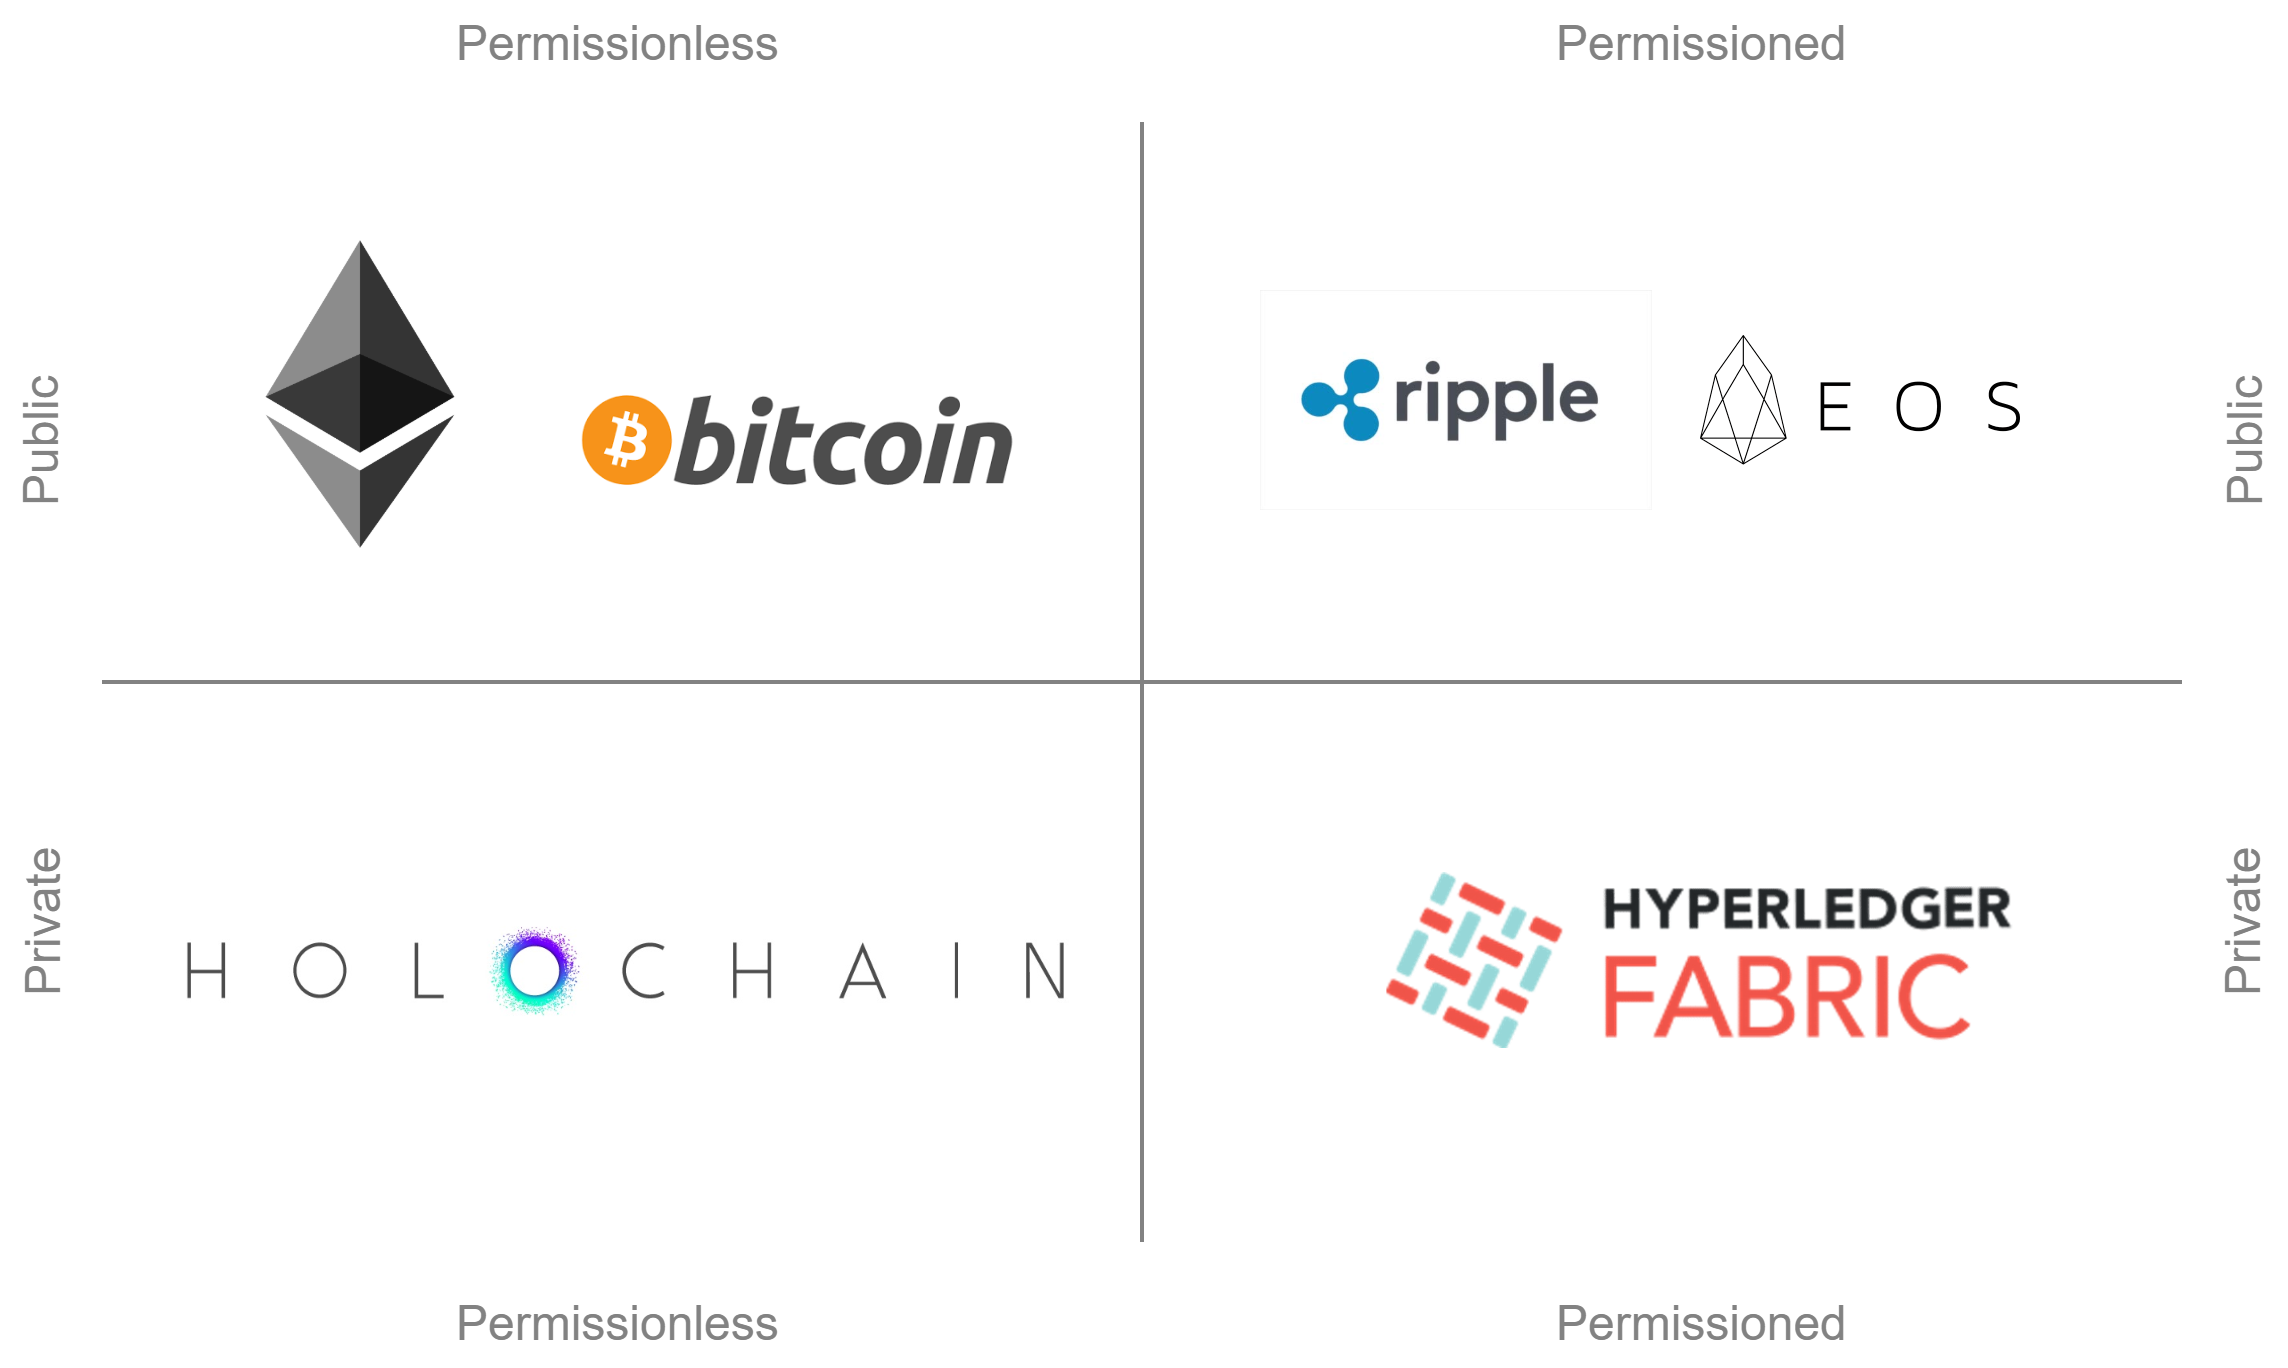
\includegraphics[width=0.8\textwidth]{gfx/taxonomy.png}
 \caption{Taxonomie von Blockchains (vgl. \cite{daniels2018})}
 \label{fig:chapter02:taxonomy}
\end{figure}

Die bekanntesten Vertreter Bitcoin und Ethereum sind öffentliche und beschränkungslose Blockchains, an denen jeder teilnehmen kann und alle Daten öffentlich einsehbar sind. Im Unternehmensumfeld wird häufig auf eine private Blockchain gesetzt, da die Zugangskontrolle zu gegebenenfalls sensiblen Daten gewährleistet wird und keine Geschäftsgeheimnisse nach Außen dringen können. Kooperationen zwischen mehreren Unternehmen werden oftmals als private, permissioned Blockchains umgesetzt, da hier jeder Kooperationspartner einen oder mehrere am Konsensverfahren teilnehmende Knoten besitzt.


\subsection{Smart-Contracts}
\label{subsec:fundamentals:dlt:smartcontracts}
Ein essentieller Bestandteil vieler Blockchains sind sogenannte Smart-Contracts. Dabei handelt es sich um Software-Code, der auf der Blockchain ("onchain") auf allen Knoten ausgeführt wird und eine Zustandsänderung meist in Form von ausgehenden Transaktionen zur Folge hat. Smart-Contracts werden in einer abgeschirmten Laufzeit-Umgebung (engl.: Runtime-Environment) ausgeführt; im Falle von Ethereum spricht man von der \ac{EVM}. Um auf Daten und Informationen außerhalb des Blockchain-Netzwerkes zugreifen zu können, können sich Smart-Contract sogenannter Oracle-Services bedienen. Dabei handelt es sich um Informationsanbieter, die zum Beispiel Wetterdaten, Lottozahlen oder Nahverkehrsinformationen an einen Smart-Contract senden, damit dieser, basierend auf den empfangenen Daten, seine Logik ausführen und die Daten verarbeiten kann. Der grundlegende Nachteil von Oracle-Services liegt in der Vertrauensfrage: Während eine Blockchain grundsätzlich mittels Konsensverfahrens die Vertrauensfrage beantwortet, obliegt dem Besitzer bzw. Betreiber eines Oracles die Macht über die Richtigkeit der Daten. Dieser Problematik kann durch den Einsatz mehrerer, mittels eines separat implementierten Konsens abgestimmter Oracle-Services entgegengewirkt werden.\\
Mit Smart-Contracts werden oftmals (allerdings nicht ausschließlich) Verträge wie Kauf- oder Mietverträge umgesetzt. Bei solchen Verträgen ist das jeweils geltende Recht eines Landes zu beachten: Die Form und der Aufbau sowie der abzubildende Inhalt eines Vertrages muss gewissen Normen entsprechen und alle benötigten Informationen enthalten, damit ein Vertrag rechtskräftig ist.


\subsection{Mutlisignatur-Wallets}
\label{subsec:fundamentals:dlt:multisig}
%http://groups.csail.mit.edu/cis/crypto/classes/6.857/papers/secret-shamir.pdf
%https://hackernoon.com/shamir-secret-sharing-vs-multi-sig-124a42bc1662
%https://www.binance.vision/de/security/threshold-signatures-explained
%https://medium.com/zengo/threshold-signatures-private-key-the-next-generation-f27b30793b
Multisignatur-Wallets sind Wallets, auf dessen Inhalt nur durch den Einsatz mehrerer Schlüssel zugegriffen werden kann. Dabei wird ein Multisignatur-Wallet von \textit{n} Schlüsseln erzeugt. Um auf das Vermögen zugreifen zu können, bedarf es der Signaturen von \textit{t von n} Schlüsseln. Dadurch können verschiedene Anwendungsfälle wie zum Beispiel Treuhandkonten (2 von 3), Zwei-Wege-Authentifizierungen und viele weitere (2 von 2) abgedeckt werden. Mutlisignatur-Wallets können entweder Teil des Blockchain-Protokolls sein (Higher fees, less privacy, not universally supported) und damit nativ unterstützt oder durch die Umsetzung mittels Smart-Contract realisiert werden. Letzteres ist dabei denkbar einfach: Es handelt sich um Code, der erst dann ausgeführt wird, wenn \textit{t von n} der hinterlegten Schlüssel unterschrieben haben. Die Höhe von \textit{t} und \textit{n} ist im Code festgelegt. Das Wallet wird demnach durch einen Smart-Contract abgebildet. Die Idee von Multisignatur-Wallets geht zurück auf das Shamir Secret Sharing Verfahren, welches im Folgenden kurz dargelegt wird:\\
\textbf{\textcolor{red}{todo}}\\
Ein großer Nachteil des Shamir Secret Sharing Verfahrens ist, dass bei der initialen Schlüsselgenerierung und bei der Entschlüsselung der vollständige private Schlüssel zusammengesetzt und damit an einem geografischen Ort vorhanden ist. Dies bietet ein gewisses Angriffspotential. Eine Weiterentwicklung des Shamir Secret Sharing Verfahrens ist das Schwellenwert-Signaturschema (engl. Threshold Signature Scheme, TSS), welches sich der \ac{MPC} bedient, wodurch der private Schlüssel niemals vollständig an einem Ort vorhanden ist. Um gemeinsam zu signieren oder entschlüsseln zu können, müssen alle beteiligten Parteien zeitlich synchron an dem Prozess teilnehmen. Das Verfahren wird im Folgenden kurz erläutert. Tiefergehende Informationen können X oder Y entnommen werden.\\
\textbf{\textcolor{red}{todo}}
Grundsätzlich verfolgen alle drei Verfahren - das Multisignatur-Wallet, das Shamir Secret Sharing Verfahren und das Schwellenwert-Signaturschema - das gleiche Ziel: Ein Geheimnis, wie zum Beispiel ein Private Key, wird auf mehrere Instanzen verteilt. Diese müssen an einem Ort zusammenkommen und ihre Teilgeheimnisse zusammenfügen, um Daten entschlüsseln oder signieren zu können. Dabei unterscheiden sich die Verfahren unter Anderem in der zeitlichen Synchronität und geografische Lage des Schlüssels.


\subsection{Konsensalgorithmen}
\label{subsec:fundamentals:dlt:consensus}
Ein Blockchain-Netzwerk ist ein dezentrales System, welches aus vielen einzelnen Knoten besteht. Damit Transaktionen und Daten über das Gesamtsystem hinweg konsistent sind, bedarf es eines Mechanismus, welcher sicherstellt, dass alle Knoten die gleichen Daten halten. Solche Mechanismen werden durch Konsensalgorithmen beschrieben. Es handlet sich dabei um ein Protokoll, welches Regeln definiert, wie und welche Daten gespeichert und welche verworfen werden. Im Folgenden werden einige bekannte Konsensverfahren genannt und kurz vorgestellt.
\begin{description}
  \item[Proof-of-Work (PoW)] Transaktionen werden durch das Lösen eines kryptografischen Puzzles (Mining) wie zum Beispiel die Ermittlung eines Hashwertes abgesichert. Ein Knoten, der eine Transaktion dem Ledger hinzufügen möchte, muss zuerst eine zufallsbasierte Berechnung durchführen, um dem Netzwerk die Validität zu beweisen. Andere Knoten können mit sehr wenig Aufwand überprüfen, ob die Berechnung korrekt war und der Knoten ehrlich gehandelt hat. Dieses Konsensverfahren ist meist mit einem hohen Stromverbrauch verbunden, da die zeitaufwändige Berechnung viele Ressourcen benötigt.
  \item[Proof-of-Stake (PoS)] Unter der Annahme, dass Knoten mit hoher finanzieller Beteiligung (Stake) ehrlich agieren, um der Plattform nicht zu schaden und ihre finanziellen Mittel nicht zu gefährden, werden diese bei der Auswahl bevorzugt, eine Transaktion dem Ledger hinzuzufügen. Dieses Verfahren ist deutlich stromsparender als PoW, allerdings durch die Miteinbeziehung des Vermögens auch ungerechter im Vergleich zu PoW.
  \item[Delegated-Proof-of-Stake (dPoS)] Dieses Verfahren ergänzt PoS um ein Delegierten-System, was die Anzahl an potentiellen Konsensknoten stark einschränkt und damit die Performance erhöht. Knoten, die bösartig handeln, können aus dem Konsens herausgewählt werden.
  \item[Practical Byzantine Fault Tolerance (PBFT)] Um in der Lage zu sein, bis zu einem Drittel an bösartigen Knoten handhaben zu können (Byzantinischer Fehler), müssen alle Knoten des Gesamtsystems bekannt sein. Dieses Verfahren löst das Konsensproblem, indem der Konsens in Runden eingeteilt wird und jede Runde Transaktionen in den Ledger übernommen werden. Indem die Knoten untereinander ihre Validierungsergebnisse austauschen kann ein Mehrheitsentscheid durchgeführt werden und damit die korrekten Transaktionen identifiziert werden.
  \item[Proof-of-Authority (PoA)] Dieses Verfahren wird meist in privaten und zugangsberechtigten Blockchains eingesetzt. Die Konsensknoten sind fest definiert und fungieren als Moderatoren des Gesamtsystems. Da kein Mining existiert, können Transaktionskosten minimal gehalten werden und das System kann aufgrund des einfachen Aufbaus des Konsens sehr gut skalieren.
\end{description}
Detailliertere Informationen sowie weitere Konsensverfahren werden von \cite{Salimitari2018ASO}, \cite{overview2017} und \cite{consensusIOT2018} vorgestellt und analysiert.


\subsection{Skalierungsansätze}
\label{subsec:fundamentals:dlt:scaling}
%https://hackernoon.com/difference-between-sidechains-and-state-channels-2f5dfbd10707
Viele Blockchain-Implementierungen stoßen schnell an ihre Grenzen \cite{overview2017}, betrachtet man die Skalierbarkeit unter realistischen Rahmenbedingungen und realen Anwendungsfällen. Steigende Anforderungen vor allem an die Transaktionsverarbeitung pro Zeitintervall \cite{Macdonald2017} (meistens \ac{TPS}) erfordern eine verbesserte Performanz und neue Lösungsansätze.\\
Als eine mögliche Antwort auf das Skalierungsproblem von Blockchains werden sogenannte State-Channels entwickelt. Ziel ist es dabei, jegliche Arten von Status-ändernden Operationen off-chain zu prozessieren, die typischerweise auf der Blockchain ausgeführt und on-chain gespeichert werden. Dadurch können die Anzahl an Zugriffen auf die Blockchain sowie die Anzahl an Transaktionen verringert und gleichzeitig die Interaktionszeit zwischen einzelnen Parteien verbessert werden. Im Kontext von Zahlungen (Payments) werden dadurch sogenannte Micro-Payments ermöglicht; bei State-Channels, die sich auf die Zahlungsabwicklung beschränken, spricht man von Payment-Channels. Diese können schneller und günstiger als normale Transaktionen erfolgen. Die Kosten solcher Micro-Payments können sehr gering gehalten werden, da nicht alle Transaktionen auf der Blockchain gespeichert werden. Die Grundidee ist dabei folgende: Alice und Bob reservieren einen Teil ihres Vermögens auf der Blockchain, sodass sie vorerst nicht darüber verfügen können und eröffnen einen Payment-Channel zueinander. Diese Transaktion, also das Eröffnen des Payment-Channels, wird auf der Blockchain gespeichert. Das Volumen des Channels, also das Vermögen, dass Alice und Bob nun zwischen einander austauschen können, entspricht der Summe der reservierten Vermögen. Ihr gewünschtes Vermögen, welches für den Payment-Channel reserviert werden soll, kann entweder mittels Multisignatur-Wallet (vgl. Kap. \ref{subsec:fundamentals:dlt:multisig}) oder Smart-Contract (vgl. Kap. \ref{subsec:fundamentals:dlt:smartcontracts}) reserviert werden. Alice und Bob haben nun einen State von jeweils 50 Euro. Anschließend können sich beide signierte off-chain Transaktionen schicken (also nicht über das Blockchain-Netzwerk). Diese Transaktionen enthalten den neuen State: Überweist Bob 10 Euro an Alice, so ändert sich der State von Alice von 50 Euro auf 60 Euro. Schickt Bob erneut eine Transaktion von 10 Euro, so ändert sich der State von Alice auf 70 Euro. Diesen Vorgang können beide nun solange wiederholen, wie sie möchten, solange sie sich in dem Volumen von 100 Euro bewegen. Zum Schließen eines Channels sendet Alice oder Bob eine Transaktion an das Blockchain-Netzwerk, welche den finalen State enthält (im Beispiel hat Alice 70 Euro und Bob 30 Euro). Für theoretisch unendlich viele Transaktionen zwischen Alice und Bob müssen lediglich die eröffnende und die schließende Transaktion des Payment-Channels on-chain gespeichert werden.\\
%https://busy.org/@bit-news/scalability-solutions-part-1
Einen weiteren, großen Vorteil liefert die durch den State-Channel ermöglichte Asynchronität von Transaktionen. Befinden sich Teilnehmer nicht im Blockchain-Netzwerk (zum Beispiel durch Konnektivitätsprobleme), so können keine Transaktionen durchgeführt werden. Hängen beispielsweise reale Aktionen wie zum Beispiel das Öffnen einer Schranke oder das Prozessieren einer Aktion mit einer Blockchain-Statusaktualisierung zusammen, so würde bei Konnektivitätsverlust der reale Prozess zum Stillstand kommen, bis die Verbindung wiederhergestellt wird. State-Channel könnten hierbei eingesetzt werden, um eine redundante Verbindung zu schaffen, die auch bei Nicht-Erreichbarkeit der Blockchain genutzt werden könnte. Einige Beispiel-Implementierungen von State-Channels sind Bitcoins Lightning Network, Ethereums Raiden Network oder die Implementierung von Neo namens Trinity.\\
Eine weitere Möglichkeit, Blockchain-Anwendungen zu skalieren, kann durch den Einsatz von Side-Chains geschaffen werden. Hierbei handelt es sich um separate Blockchains, die parallel zur Haupt-Blockchain (auch oft Eltern-Blockchain oder Main-Chain genannt) laufen. Um eine Side-Chain zu eröffnen, muss zunächt der Beweis erbracht werden, dass alle Assets, deren Status in der Side-Chain verändert werden sollen, auf der Main-Chain gesperrt oder reserviert sind, sodass der Eigentümer temporär nicht über diese verfügen kann. Diese gesperrten Assets können anschließend in die Side-Chain transferiert werden. Dort kann der Status verändert werden; beispielsweise kann eine Geld-Transaktion durchgeführt werden. Soll ein Asset zurück auf die Main-Chain transferiert werden, so muss der Beweis erbracht werden, dass dieses Asset auf der Side-Chain gesperrt wurde. Dadurch werden Effekte wie das Double-Spending verhindert. Ähnlich wie bei State-Channels handelt es sich auch bei Side-Chains um einen Skalierungsansatz auf Layer-2 der Blockchain-Architektur. Das bedeutet, dass diese Ansätze nicht direkt auf der Blockchain selbst (Layer-1) ausgeführt werden.

\subsection{Dezentrale Identitäten}
\label{subsec:fundamentals:dlt:did}
Eine Identität zeichnet sich durch eine Menge von Informationen, Daten und Eigenschaften aus, die diese eindeutig identifizieren. Nur der Inhaber einer Identität kann mit dieser auch agieren, da er der einzige ist, der Zugriff auf die geschützten Informationen hat, die das Innehaben einer Identität bestätigen. Diese können zum Beispiel ein Passwort, eine Geburtsurkunde, ein Fingerabdruck oder Ähnliches sein.\\
Eine dezentrale Identität ist eine neuartige Technologie, die es dem Inhaber einer solchen erlaubt, seine Identität digital, dezentral und sicher durch den Einsatz asymmetrischer Verschlüsselung selbst zu verwalten. Sie ist kryptografisch verifizierbar und der Inhaber entscheidet selbst, welche Informationen er teilen möchte und welche nicht. Das \ac{W3C} entwickelt aktuell (Stand: Dezember 2019) einen Industrie-Standard, der zur Verifizierung und Authentifizierung persönlicher Informationen vor Dritten im Web 3.0 eingesetzt werden soll und sich derzeit in der Version 1.0 befindet \cite{did2019}. Eine dezentrale Identität besteht aus einer \ac{DID}, welche weltweit einzigartig ist, und einem dazugehörigen DID-Dokument, welches Informationen über den beschriebenen Gegenstand enthält. Die folgenden Beispiele zeigen eine \ac{DID} und ein dazugehöriges DID-Dokument (entnommen aus \cite{did2019}).

\begin{lstlisting}[caption=Beispiel einer DID,label=listing:did]
did:example:123456789abcdefghi
\end{lstlisting}

\begin{lstlisting}[caption=Beispiel eines DID-Dokuments,label=listing:did_document]

{
  "@context": "https://www.w3.org/ns/did/v1",
  "id": "did:example:123456789abcdefghi",
  "authentication": [{

    "id": "did:example:123456789abcdefghi#keys-1",
    "type": "RsaVerificationKey2018",
    "controller": "did:example:123456789abcdefghi",
    "publicKeyPem": "-----BEGIN PUBLIC KEY...END PUBLIC KEY-----\r\n"
  }],
  "service": [{

    "id":"did:example:123456789abcdefghi#vcs",
    "type": "VerifiableCredentialService",
    "serviceEndpoint": "https://example.com/vc/"
  }]
}
\end{lstlisting}

Durch den Einsatz von Blockchain-Technologie können \ac{DID}s manipulationssicher, hochverfügbar und für jeden zugänglich gespeichert werden. Die \ac{DID} besteht aus drei Teilen: Zunächst dem Schlüsselwort "did", welches beschreibt, dass es sich um eine \ac{DID} handelt. Anschließend folgt die DID-Methode (im Beispiel: "example"), die definiert, wie die \ac{DID} aufzulösen und weitere Informationen zu dieser Identität zu finden sind. Der letzte Teil ist eine ID ("123456789abcdefghi"), die für jede Methode einzigartig ist und somit eindeutig ermittelt werden kann.\\
Darüber hinaus existieren sogenannte \ac{VC}, die einer \ac{DID} von vertrauenwürdigen Instanzen ausgestellt werden können. Dabei handelt es sich um verifizierbare Berechtigungsnachweise. Der Aussteller bescheinigt dem Empfänger eine bestimmte Eigenschaft und stellt einen Service-Endpoint zur Verfügung, an dem ein Dritter diesen \ac{VC} verifizieren kann. So kann zum Beispiel eine Universität mit ihrer eigenen \ac{DID} "did:hda:12345" einem Student "did:test:sebastiankanz" ein \ac{VC} ausstellen, welches dem Student bescheinigt, aktuell an der Universität eingeschrieben zu sein. Möchte sich der Student nun an der Universitätsbibliothek authentifizieren, so kann er dort das \ac{VC} der Universität vorzeigen und bekommt Zugriff auf die Bibliotheksausleihe. Die Bibliothek kann das \ac{VC} verifizieren, indem es unter der Methode "hda" die Universität identifiziert und anschließend die Signaturen überprüft.

\subsection{Blockchain im Kontext des OSI-Referenzmodells}
\label{subsec:fundamentals:dlt:osi}
Das \ac{OSI} Modell gilt seit Mitte der 80er-Jahre als Standard zur Einordnung von Netzwerkprotokollen. Es wurde von der \ac{ISO} entwickelt und besteht aus sieben Schichten (\cite{OSI1980}, \cite{osi2014}):
\begin{description}
  \item[Physical Layer] Die Übertragung des Bit-Datenstroms über ein physikalisches Medium (Hardware) findet auf dieser Ebene statt.
  \item[Data Link Layer] Diese Schicht kapselt Daten in Datenframes; es werden grundlegende Funktionalitäten zur Fehlererkennung und Fehlerbehebung bereitgestellt. Bekannte Protokolle dieser Ebene sind zum Beispiel Ethernet und \ac{ARP}.
  \item[Network Layer] Diese Schicht kapselt Daten in Datenpaketen und implementiert Sequenznummern, Flusskontrolle und Funktionalitäten fürs Routing.
  \item[Transport Layer] Diese Schicht ist zuständig für die Ende-zu-Ende Übermittlung von Daten, die sie vom Session Layer empfängt. Die Daten werden in sogenannte Segmente unterteilt und über das Netzwerk versendet und auf der Empfängerseite ebenfalls von der Transport-Schicht wieder zusammengesetzt.
  \item[Session Layer] Kommunikationskanäle werden auf dieser Schicht geöffnet, geschlossen und verwaltet und heißen Sessions.
  \item[Presentation Layer] Diese Schicht ist zuständig für Datenkonvertierungen, -kompressionen und stellt Funktionalitäten wie Ver- und Entschlüsselung bereit.
  \item[Application Layer] Diese Schicht stellt die Schnittstelle zum Benutzer dar.
\end{description}

Bei einem dezentralen System wie \ac{DLT}, welches über ein Netzwerk kommuniziert, liegt es nahe, eine Einordnung in das \ac{OSI} Modell durchzuführen. Dazu werden die verschiedenen Bestandteile eines \ac{DLT}s vorgestellt und den Schichten des \ac{OSI} Modells zugeordnet. Die Schichten eins bis drei (Physical, Data Link und Network) werden hierbei nicht betrachtet, da die Kommunikation über das Internet erfolgt und demnach auf bekannten Protokollen aufgebaut wird (Ethernet, IP).

Eine Blockchain basiert auf einem \ac{P2P}-Netz, in dem alle Knoten miteinander verbunden sind und miteinander kommunizieren können. Diese Kommunikation geschieht nach dem Ende-zu-Ende Prinzip und nicht nach dem Punkt-zu-Punkt Prinzip. Die \ac{P2P}-Kommunikation erfolgt meist über die entsprechenden Transportprotokolle TCP oder UDP, welche Daten als Segmente zwischen Sender und Empfänger austauschen. Demnach findet die \ac{P2P}-Kommunikation auf dem Transport-Layer (Schicht 4) statt.\\
Der Konsensalgorithmus legt zum einen fest, welche Knoten am Konsensverfahren partizipieren dürfen und welche nicht. Dazu werden Verbindungen zu anderen Knoten aufgebaut und ggfs. wieder geschlossen. Zum anderen wird definiert, welchem Schema die Kommunikation folgt. Eingehende Datensegmente der \ac{P2P}-Schicht werden entgegengenommen und in Form von Transaktionen gemäß der Konsensregeln verarbeitet. Die Ergebnisse werden wiederum an die \ac{P2P}-Schicht zurückgespiegelt und über das Netzwerk an die anderen Knoten publiziert. Diese Vorgänge sind in den Session-Layer des \ac{OSI}-Modells einzuordnen.\\
Die virtuelle Maschine einer Blockchain sorgt dafür, dass die Verarbeitungsschritte auf allen Knoten zum selben Ergebnis führen. Dazu werden Smart-Contracts aus Transaktionen extrahiert, in Byte-Code übersetzt und in separierten Laufzeitumgebungen ausgeführt. Verschlüsselte Nutzdaten von Transaktionen werden ebenfalls in dieser Laufzeitumgebung entschlüsselt. Die Funktionen der Smart-Contracts werden der nächst-höheren Schicht zur Verfügung gestellt. Darüber hinaus werden Daten, die in Byte-Form aus Smart-Contracts entstehen, konvertiert und in Form von Transaktionen an die untere Ebene weitergereicht. Diese Funktionalitäten können in den Presentation-Layer (Schicht 6) eingeordnet werden.\\
Die Schittstellen zum Benutzer stellen Top-Level-\ac{API}s dar, über die der Benutzer mitels Transaktionen mit der Blockchain kommunizieren kann. Sendet ein Benutzer eine Transaktion an einen Smart-Contract, kann dieser Aktionen triggern und Daten zurück an den Benutzer senden. Darüber hinaus gibt es dApps, ein Zusammenschluss mehrerer, zusammenarbeitender Smart-Contracts, auf dessen Daten der Benutzer beispielsweise mittels Webanwendung über seinen Browser zugreifen kann. Zusammen können diese Funktionalitäten dem Application-Layer (Schicht 7) zugeordnet werden.\\

In Abbildung \ref{fig:chapter02:osi_blockchain} werden die zugeordneten Schichten der Blockchain noch einmal aufgezeigt und mit den sieben Schichten des \ac{OSI}-Modells dargestellt.

\begin{figure}[htbp]
 \centering
 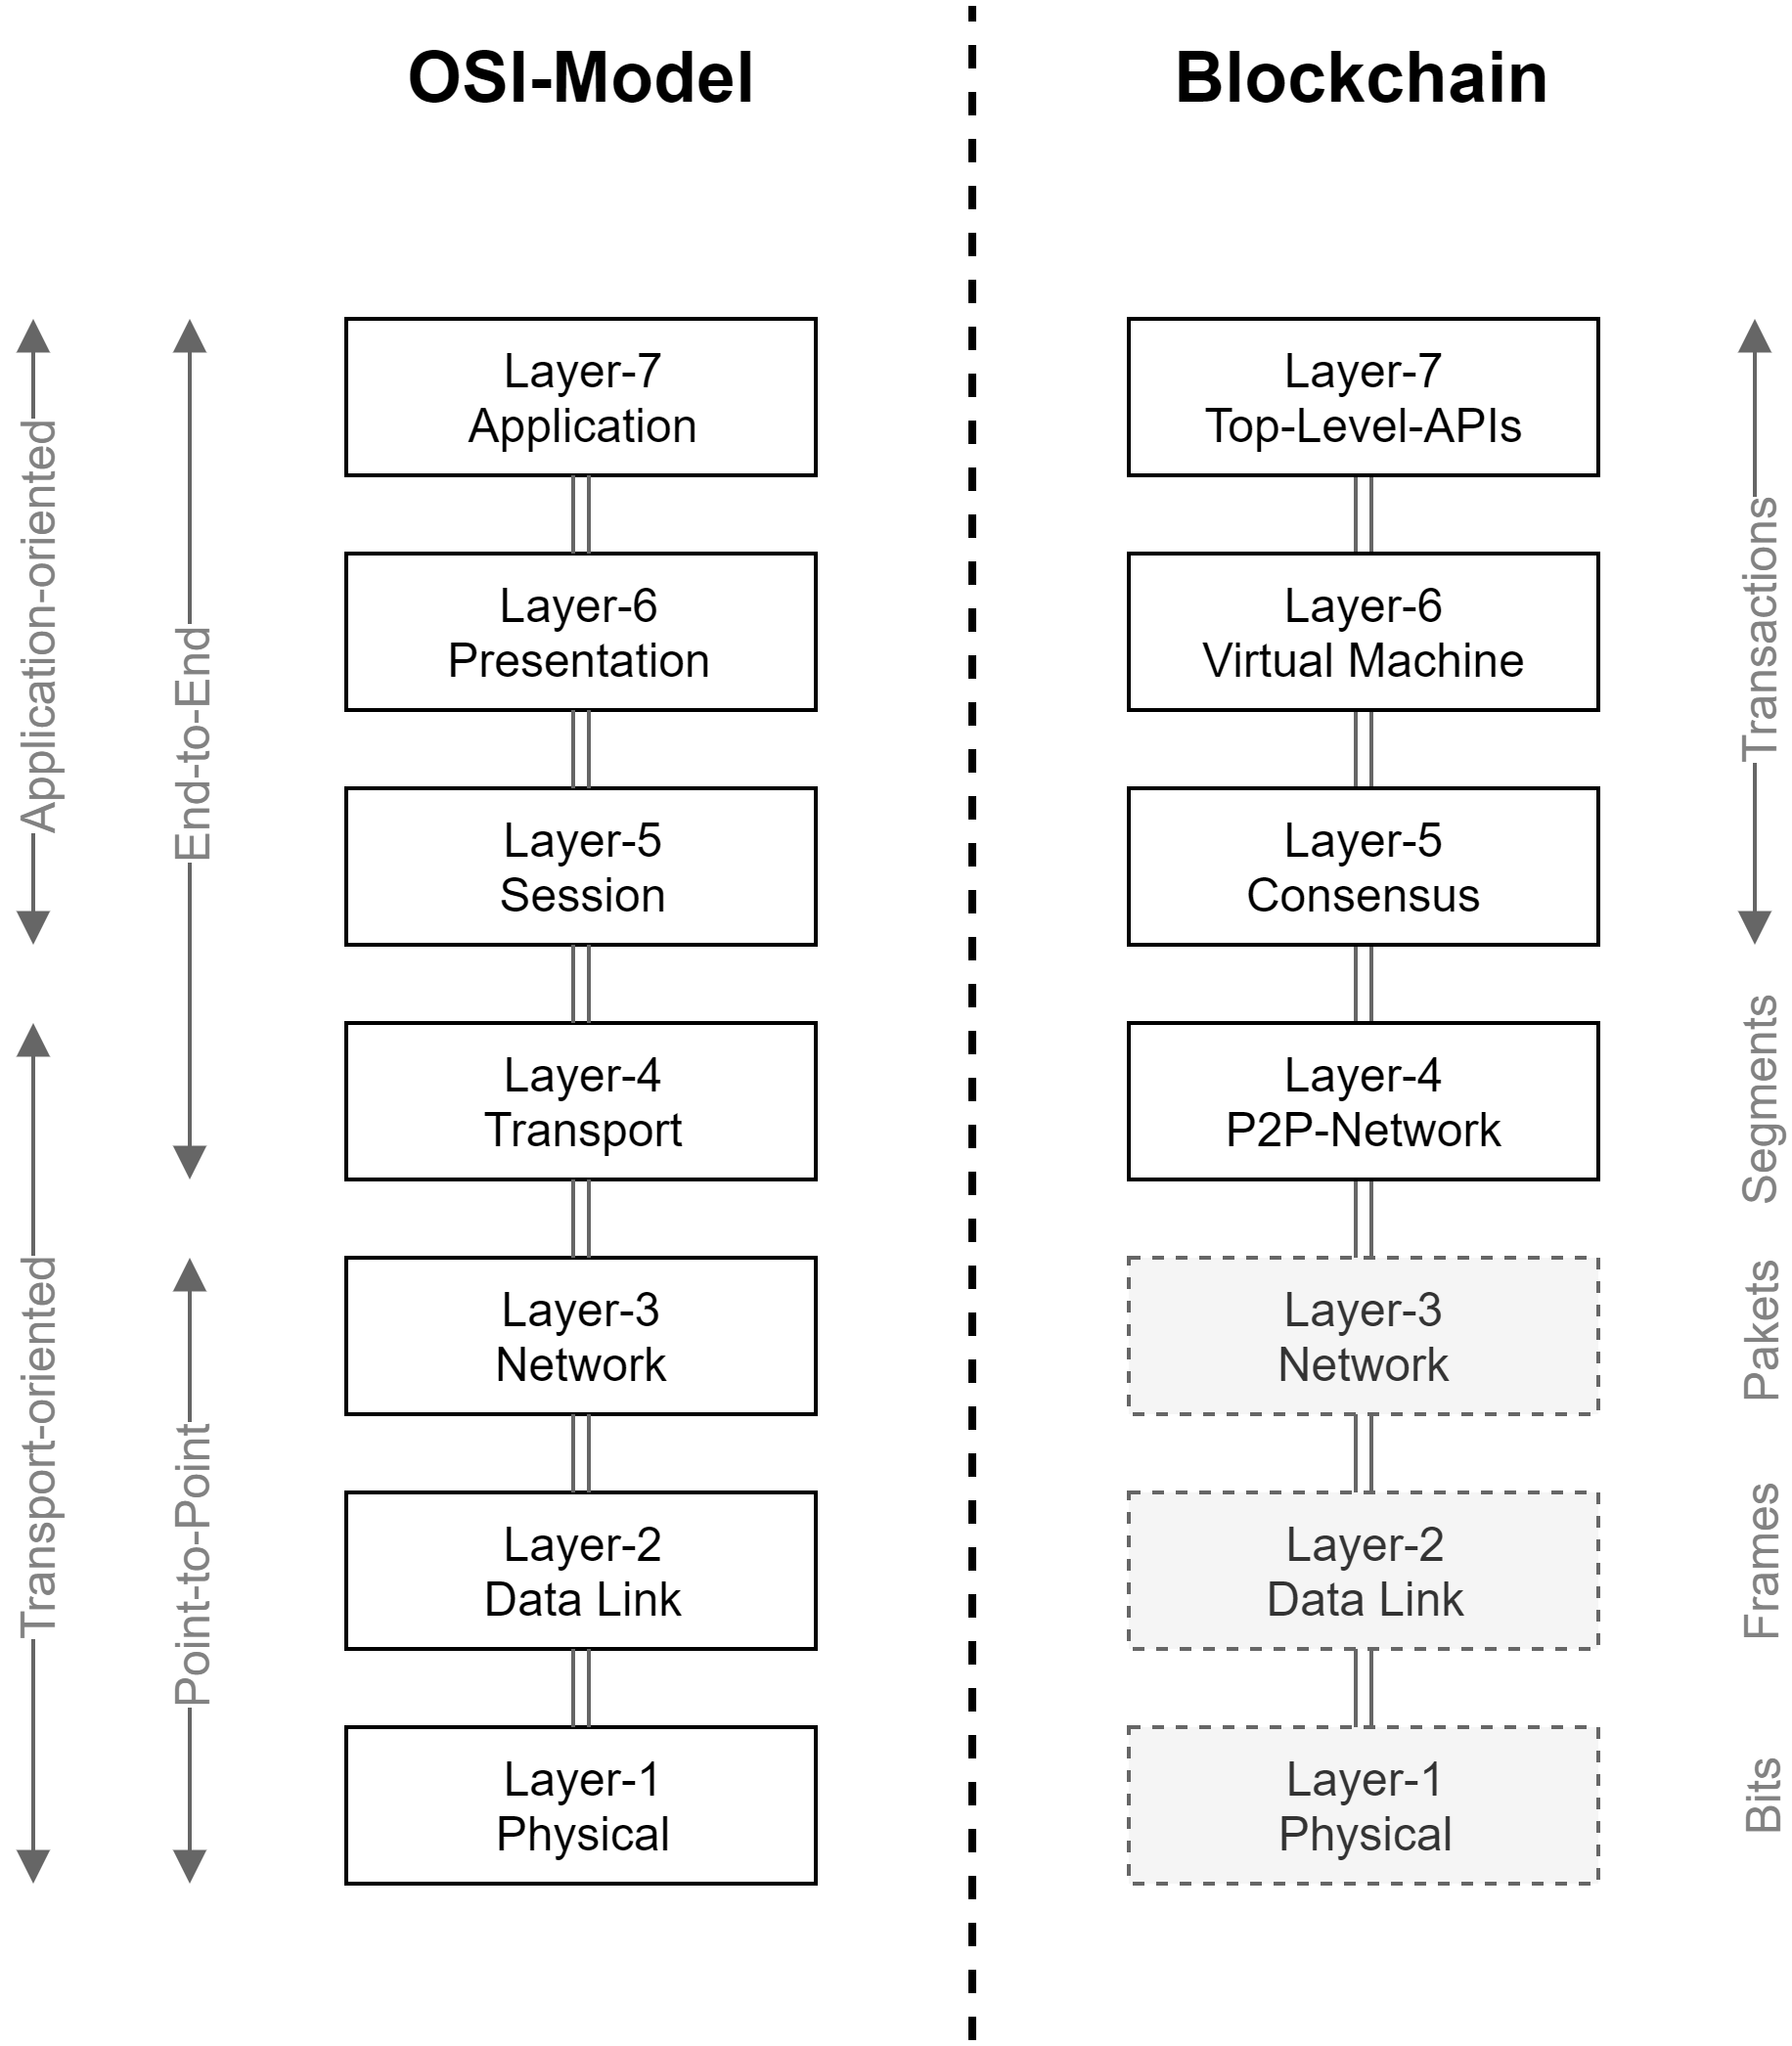
\includegraphics[width=0.6\textwidth]{gfx/osi_blockchain.png}
 \caption{Die Blockchain-Layer im Konext des OSI-Modells}
 \label{fig:chapter02:osi_blockchain}
\end{figure}

Der Duden definiert den Begriff Protokoll als \glqq Festlegung von Standards und Konventionen für eine reibungslose Datenübertragung zwischen Computern\grqq. Ein Kommunikationsprotokoll ist gemäß des Gabler Wirtschaftslexikons \glqq eine Übermittlungsvorschrift bei der Datenübertragung, die die gesamten Festlegungen für Steuerung und Betrieb der Datenübermittlung in einem Übermittlungsabschnitt [...] umfasst\grqq. Diese Definitionen zusammen mit der Einordnung der Blockchain-Technologie in das \ac{OSI}-Modell machen deutlich, dass es sich bei dabei um ein Kommunikationsprotokoll handelt. Zusammen mit der Zahlungsabwicklung und der Abbildung von Eigentumsverhältnissen beziehungsweise Eigentumsübergängen spricht man auch von einem sogenannten \glqq Value Exchange Protcol\grqq \cite{bheemaiah2015}.\\
Durch die Einordnung in das \ac{OSI}-Modell kann auch die Sinnfrage beantwortet werden, weshalb die Blockchain-Technologie anstatt herkömmlicher Ansätze eingesetzt werden sollte: Betrachtet man die Technologie objektiv, abseits des Hypes und des Anwendungsfalls der Kryptowährungen, so erkennt man eine junge Technologie mit hohem Potenzial. Die Blockchain als Kommunikationsprotokoll gibt dem modernen Softwareentwickler umfangreiche Werkzeuge und Out-of-the-Box Funktionalität über vier Schichten des \ac{OSI}-Modells hinweg an die Hand. Eine dezentrale Plattform mit integrierter Datenbank, Security, Ver- und Entschlüsselung,\ac{P2P}-Netzwerkkommunikation, Entwicklungs- und Laufzeitumgebung für dezentrale Anwendungen, sicherer Zahlungsabwicklung und hoher Verfügbarkeit ist oftmals per Knopfdruck binnen Sekunden erstellt. Alle diese Bestandteile und Funktionalitäten sind in der technischen Spezifikation einer jeden Blockchain in Form eines Kommunikationsprotokolls enthalten und definiert.

%
% Section: IOT
%
\section{Internet of Things}
\label{sec:fundamentals:iot}
Der Begriff Internet der Dinge - kurz \ac{IOT} - ist ein Sammelbegriff und bezeichnet die Vernetzung von Gegenständen untereinander (meist über das Internet). Es wird eine autonome \ac{M2M}-Kommunikation ermöglicht, die wiederum den Automatisierungsgrad in dem jeweiligen Einsatzgebiet erhöht. Das bedeutet, dass die Kommunikation zwischen den \ac{IOT}-Geräten selbst erfolgt, also ohne das Eingreifen eines Menschen. Nach \cite{deloitte2018} lässt sich das Themenfeld \ac{IOT} in zwei Bereiche untergliedern: \ac{CIOT} und \ac{IIOT}. Während \ac{CIOT} Anwendungen im privaten Umfeld sieht - vor allem geht es hier um Smart-Home und den damit verbundenen Applikationen - so fokussiert sich \ac{IIOT} auf den kommerziellen Bereich und versucht Anwendungen im deutlich größeren Stil zu entwickeln: Die Bereiche Automotive, Energie und Supply-Chain sind hierbei einige wichtige Vertreter. Konkrete Anwendungsbereiche und weitere Beispiele für beide \ac{IOT}-Bereiche werden im Abschnitt \ref{subsec:fundamentals:iot:usecases} erläutert.\\


\subsection{Anwendungsbereiche im Kontext DLT}
\label{subsec:fundamentals:iot:usecases}
Smart-City (Power-Management, Car Sharing, Parking, Traffic)
Smart-Factory (Automation)
Smart-Home (Door-locks, Security, Gardening, Lighting)
Smart-People (Fitness-Tracker, Pulse-Meter, Step-Counter)
Supply-Chain
Automotive (Connected Cars, Traffic)

\textbf{\textcolor{red}{todo}}
IOT-Bereiche mit Anwendungsbeispielen - Echtzeitanwendungen,


\subsection{Vorteile durch den Einsatz von DLT}
\label{subsec:fundamentals:iot:dlt_iot}
Die grundlegenden Vorteile, die ein Einsatz der Blockchain-Technologie mit sich bringt, wurden in Abschnitt \ref{subsec:fundamentals:dlt:osi} aufgezeigt. Darüber hinaus formulierten Christidis et al. (\cite{SCIOT2016}) den IOT-Sachverhalt aus Sicht des Herstellers und des Kunden sehr treffend:\\
\glqq From the manufacturer's side, the current centralized model has a high maintenance cost consider the distribution of software updates to millions of devices for years after they have been long discontinued. From the consumer's side, there is a justified lack of a trust in devices that phone home in the background and a need for a security through transparency approach.\grqq\\
Christidis et al. nennen zwei zentrale Kerneigenschaften eines Distributed Ledgers: Zum einen die Verteilung und die einfache Anbindung und Erreichbarkeit von \ac{IOT}-Geräten, die die Wartung seitens des Herstellers erleichtern können. Zum anderen sprechen die Autoren die Vertrauensfrage seitens der Kunden in Bezug auf Datensicherheit und Privatsphäre an. Hier kann die Blockchain-Technologie \glqq Sicherheit durch Transparenz\grqq erzielen und für eine größere Akzeptanz sorgen.\\
Der Einsatz von Blockchain-Technologie ist allerdings nicht immer ratsam oder möglich. So kann beispielsweise aufgrund des Anwendungsfalls oder aufgrund von technischen Beschränkungen und Gegebenheiten der Einsatz eines \ac{DLT}s im \ac{IOT}-Umfeld unvorteilhaft sein. Ersteres könnte zum Beispiel eine Smart-Home Anwendung sein, die eine Temparaturregelung und Überwachung der eigenen vier Wände vorsieht. Ein dezentraler Ledger wäre hier überdimensioniert und für diesen Zweck überqualifiziert. Der Aufwand stünde in keinem Verhältnis zum Nutzen. Darüber hinaus zeigt dieser \ac{IOT}-Anwendungsfall auch keine Charakteristika einer \ac{DLT}-Anwendung auf: Es handelt sich um eine einzige beteiligte Partei in einem vertrauten Umfeld mit nur wenig Endgeräten. Auf der anderen Seite können technsiche Hürden den Einsatz von \ac{DLT} verhindern. Gerade im Automotive-Bereich ist die Verarbeitung von Sensor- und Aktordaten in Echtzeit ein kritischer Punkt. Dezentrale Ledger eigenen sich hierzu nicht, da sie nicht in der Lage sind, zeitkritische Anwendungen zu betreiben.\\
Es wird deutlich, dass die Beschaffenheit des \ac{IOT}-Anwendungsfalls sehr entscheidend dazu beiträgt, ob der Einsatz einer Blockchain-Lösung sinnvoll sein kann oder nicht.

\subsection{Digitaler Zwilling}
\label{subsec:fundamentals:iot:digitaltwins}
Ein digitaler Zwilling (engl. Digital Twin) ist nach \cite{deloitte2018} eine virtuelle Kopie physikalischer Objekte. Diese besteht aus definierten Datenstrukturen, einem \ac{UI}, welches relevante Daten visualisiert, IT-Komponenten zur Statusaktualisierung und vorhandener Konnektivität. Digitale Zwillinge werden in automatisierten IT-Prozessen benötigt, die sie als Schnittstelle zwischen physischer Welt und dessen digitalen Pendant fungieren. Der Zustand eines physikalischen Objekts wird in den digitalen Zwilling gespiegelt, welcher wiederum eine digitale Zustandsüberwachung und die Manipulation seines physischen Gegenstücks ermöglicht \cite{deloitte2018}. Der Ansatz von digitalen Zwillingen und die Thematik \ac{IOT} haben gegenseitig enormen Einfluss aufeinander und befähigen einander zu neuen Anwendungsfällen. Diese können unter Anderem die Abbildung von Fabriken und Maschinen in digitale Automatisierungsprozesse sein, indem die Geräte und Teile mit Sensoren, Konnektivität und einer Steuerungslogik ausgestattet werden. Dadurch können Predictive Maintance, Bedarfsplanungen und Prozessoptimierungen durchgeführt werden.
